\documentclass[11pt,a4paper]{ctexart}
\usepackage[margin=2.4cm]{geometry}
\usepackage{amsmath,amssymb,amsthm}
\usepackage{booktabs}
\usepackage{graphicx}
\usepackage{xcolor}
\usepackage{enumitem}
\usepackage{hyperref}
\hypersetup{colorlinks=true,linkcolor=blue!50!black,citecolor=blue!50!black,urlcolor=blue!50!black}
\setlength{\emergencystretch}{2em}

\newtheorem{theorem}{定理}
\newtheorem{proposition}{命题}
\newtheorem{lemma}{引理}
\newtheorem{corollary}{推论}
\theoremstyle{definition}
\newtheorem{remark}{注}
\newtheorem{definition}{定义}
\newtheorem{conjecture}{猜想}
\newtheorem{statusbox}{状态}

\newcommand{\proved}{\textcolor{green!45!black}{\textbf{[已证明]}}}
\newcommand{\loword}{\textcolor{orange!80!black}{\textbf{[低阶精确检验]}}}
\newcommand{\numeric}{\textcolor{blue!70!black}{\textbf{[数值证据]}}}
\newcommand{\conj}{\textcolor{red!70!black}{\textbf{[猜想/未闭合]}}}
\newcommand{\Tr}{\operatorname{Tr}}
\newcommand{\Hom}{\operatorname{Hom}}
\newcommand{\End}{\operatorname{End}}
\newcommand{\id}{\operatorname{id}}
\newcommand{\TrT}{\widetilde{\Tr}}
\newcommand{\E}{\mathbb{E}}
\newcommand{\C}{\mathbb{C}}
\newcommand{\R}{\mathbb{R}}
\newcommand{\ph}{\varphi}
\newcommand{\Frec}{F_{\rm rec}}
\newcommand{\Nalg}{S_{\rm alg}}
\newcommand{\Nqtr}{S_{\rm qtr}}
\newcommand{\dist}{\operatorname{dist}}
\newcommand{\Page}{\mathrm{Page}}
\newcommand{\dd}{\mathrm{d}}
\newcommand{\ii}{\mathrm{i}}
\newcommand{\ee}{\mathrm{e}}

\title{\bfseries Fibonacci 融合约束下的 Page 转折与量子信息可恢复性{}\\[4pt] \large 题二研究报告}
\author{研究计算报告（可复现；脚本见附录~\ref{app:code}）}
\date{2026-09-23}

\begin{document}
\maketitle

\begin{abstract}
本报告在题面给定的 random-code toy model 中，对以下问题给出完整的可核验结果并加以验证：（一）两种明确给定的熵（$S_{\rm alg}$ 与 $S_{\rm qtr}$）的精确有限维期望值、二阶 replica moment 及其 $N\to\infty$、$N_R-N_B=O(1)$ 渐近展开（含首个非平凡修正）；（二）由 Stiefel 矩精确计算 $\E\,\Tr C_{QB}^2$，其中 $C_{QB}=\rho_{QB}-\frac{I_Q}{k}\otimes\rho_B$，并由此给出约束 $F_{\rm rec}$（式 \eqref{eq:Q2}）的非空洞上下界（$F_{\rm rec}\ge F_{\rm Petz}$ 的显式下界与 SDP 对偶上界，两者均可对给定 $V$ 精确计算）；（三）对候选临界变量 $\Xi=N_R-N_B-\log_{\ph}k$ 的定量检验。主要结论：$\E\,\Tr C_{QB}^2$ 有精确闭式
\[
\E\,\Tr C_{QB}^2=\frac{(k^2-1)\,(D B-A)}{k^2\,D\,(D^2-1)},\qquad
A=\sum_a m_a^2n_a,\quad B=\sum_a m_an_a^2,\quad D=\sum_a m_an_a,
\]
并且在 $N\to\infty$、$\delta=N_R-N_B$ 固定时，
$\E\,\Tr C_{QB}^2=\frac{k^2-1}{k^2}\,\frac{2\ph}{\sqrt5}\,\ph^{-N_R}\,(1+O(\ph^{-2N_B}))$。
数值（CPTP 优化）表明：恢复转折由 $\Xi$ 控制，且 $1-\Frec\approx 0.20\,\ph^{-\Xi}$（$N\ge11$，8 个数据点，$c=0.200\pm0.019$）；候选变量 $\Xi$ 显著优于 $N_R-N_B-2\log_\ph k$ 与不含 $N_B$ 的变量。两种熵的 Page 转折都在 $N_R=N_B$，与 $k$ 无关，因此\textbf{熵的 Page 转折不能单独决定 $F_{\rm rec}$ 的转折}。此外我们证明：由于 $R$ 与 $B$ 共享融合扇区标签，题面定义的信道 $\mathcal N_R,\mathcal N_B$ 恰为一对互补信道，扇区退相干是自动的而非额外损失。

\medskip
\noindent 阅读约定：全文用 \proved{} 标记已给出证明的命题；\loword{} 标记精确低阶计算/精确公式的有限维检验；\numeric{} 标记数值证据；\conj{} 标记猜想或未闭合步骤。未使用的代码均不声称运行。
\end{abstract}

\tableofcontents

\section{模型、记号与三条结构事实}
\label{sec:setup}

\subsection{融合空间维数与分块}

取 unitary Fibonacci 融合范畴：$1\otimes a=a$，$\tau\otimes\tau=1\oplus\tau$，$d_1=1$，$d_\tau=\ph=\frac{1+\sqrt5}{2}$；题面给定的 $F$ 矩阵
$F^{\tau\tau\tau}_\tau=\begin{pmatrix}\ph^{-1}&\ph^{-1/2}\\ \ph^{-1/2}&-\ph^{-1}\end{pmatrix}$
是 unitary 且对称的（数值检验 $F^2=I$）。本题不涉及 braiding。

对 $n\ge 0$ 记
\[
A_n:=\dim\Hom(1,\tau^{\otimes n}),\qquad B_n:=\dim\Hom(\tau,\tau^{\otimes n}),
\]
由融合规则 $A_n=B_{n-1}$，$B_n=A_{n-1}+B_{n-1}$，$A_0=1,\ B_0=0$。于是（按 Fibonacci 数 $F_0=0,F_1=1$）
\[
A_n=F_{n-1}\ (n\ge1),\qquad B_n=F_n .
\]
对切分 $N=N_R+N_B$，定义
\[
m_1=A_{N_R}=F_{N_R-1},\quad m_\tau=B_{N_R}=F_{N_R};\qquad
n_1=A_{N_B}=F_{N_B-1},\quad n_\tau=B_{N_B}=F_{N_B}.
\]
由 $\Hom(1,\tau^{\otimes N})\cong\bigoplus_a\Hom(a,\tau^{\otimes N_R})\otimes\Hom(a,\tau^{\otimes N_B})$ 得恒等式
\[
D_N:=\sum_{a\in\{1,\tau\}}m_an_a=A_{N_R}A_{N_B}+B_{N_R}B_{N_B}=F_{N-1},
\]
以及
\[
D_R:=\sum_am_a=F_{N_R+1},\qquad D_B:=\sum_an_a=F_{N_B+1}.
\]
以上恒等式已对 $N_R,N_B\le 8$ 全部符号验证 \proved{}（脚本 \texttt{fib\_setup.py}）。表~\ref{tab:fib} 给出后文用到的若干具体数据。

\begin{table}[t]\centering
\caption{小规模 $(N_R,N_B)$ 的扇区数据。$D=F_{N-1}=m_1n_1+m_\tau n_\tau$，$D_R=F_{N_R+1}$，$D_B=F_{N_B+1}$。}
\label{tab:fib}
\begin{tabular}{ccccccccc}
\toprule
$(N_R,N_B)$ & $N$ & $m_1$ & $m_\tau$ & $n_1$ & $n_\tau$ & $D$ & $D_R$ & $D_B$\\
\midrule
$(2,2)$ & 4 & 1 & 1 & 1 & 1 & 2 & 2 & 2\\
$(3,2)$ & 5 & 1 & 2 & 1 & 1 & 3 & 3 & 2\\
$(3,3)$ & 6 & 1 & 2 & 1 & 2 & 5 & 3 & 3\\
$(4,3)$ & 7 & 2 & 3 & 1 & 2 & 8 & 5 & 3\\
$(4,4)$ & 8 & 2 & 3 & 2 & 3 & 13 & 5 & 5\\
$(5,4)$ & 9 & 3 & 5 & 2 & 3 & 21 & 8 & 5\\
$(6,5)$ & 11 & 5 & 8 & 3 & 5 & 55 & 13 & 8\\
$(8,8)$ & 16 & 13 & 21 & 13 & 21 & 987 & 34 & 34\\
\bottomrule
\end{tabular}
\end{table}

\subsection{结构事实 I：$\mathcal N_R$ 与 $\mathcal N_B$ 恰为互补信道，扇区退相干是自动的}
\label{ssec:complement}

题面把 $V:\C^k\to\mathcal H_N^1$ 从 $D_N\times D_N$ Haar unitary 的前 $k$ 列取样，并把信道定义为按扇区取偏迹：
\[
\mathcal N_R(\rho)=\bigoplus_a\Tr_{\mathcal H_B^a}\!\big(P_aV\rho V^\dagger P_a\big),\qquad
\mathcal N_B(\rho)=\bigoplus_a\Tr_{\mathcal H_R^a}\!\big(P_aV\rho V^\dagger P_a\big).
\]
在 $L$ 与 neutral reference $Q$ 的最大纠缠态 $|\Phi_k\rangle_{QL}=\frac1{\sqrt k}\sum_j|j\rangle_Q|j\rangle_L$ 下，题面定义的最佳 entanglement recovery fidelity 为
\begin{equation}\label{eq:Q2}
\boxed{\ \Frec(V)=\sup_{\mathcal D}\ \langle\Phi_k|_{QL}\Big[\id_Q\otimes\big(\mathcal D\circ\mathcal N_R\big)\Big]\big(|\Phi_k\rangle\langle\Phi_k|\big)\Big|\Phi_k\rangle_{QL}\ }
\end{equation}
其中上确界取遍从直和输出代数 $\bigoplus_a\End(\mathcal H_R^a)$ 到 $L$ 的任意 CPTP 映射 $\mathcal D$（可使用 neutral ancilla，但不额外提供非平凡拓扑荷资源）。
\begin{proposition}[补全性]\proved{}\label{prop:compl}
对任意 $\rho\in\End(\C^k)$，
\[
\mathcal N_R(\rho)=\Tr_{\mathcal H_B}\!\big(V\rho V^\dagger\big),\qquad
\mathcal N_B(\rho)=\Tr_{\mathcal H_R}\!\big(V\rho V^\dagger\big),
\]
其中 $\mathcal H_R=\bigoplus_a\mathcal H_R^a$、$\mathcal H_B=\bigoplus_a\mathcal H_B^a$。换言之，题面定义中的直和结构并不引入额外的“扇区退相干”损失；$(\mathcal N_R,\mathcal N_B)$ 是等距 $V$ 的精确互补信道对。
\end{proposition}
\begin{proof}
只需说明 $\Tr_{\mathcal H_B}(V\rho V^\dagger)$ 自动是分块对角的。一般地，对算子 $O$ 在 $\mathcal H_R\otimes\mathcal H_B=\bigoplus_{a,a'}\mathcal H_R^a\otimes\mathcal H_B^{a'}$ 上，
$\langle a\mu|\Tr_{\mathcal H_B}O|a'\mu'\rangle=\sum_{b}\langle a\mu,b|O|a'\mu',b\rangle$，其中 $b\in\mathcal H_B=\bigoplus_c\mathcal H_B^c$。对 $O=|v\rangle\langle v'|$，$|v\rangle=\sum_{c,\lambda,\nu}X^{(v)}_{c\lambda\nu}|c\lambda\rangle_R|c\nu\rangle_B$，有 $\langle a\mu,b|v\rangle\neq0\Rightarrow b\in\mathcal H_B^a$，而 $\langle v'|a'\mu',b\rangle\neq0\Rightarrow b\in\mathcal H_B^{a'}$，故 $a\ne a'$ 时该矩阵元为零。于是 $\Tr_{\mathcal H_B}(V\rho V^\dagger)=\bigoplus_a\Tr_{\mathcal H_B^a}(P_aV\rho V^\dagger P_a)$，即 $\mathcal N_R$ 的表达式。$\mathcal N_B$ 同理。
\end{proof}
\begin{remark}
命题~\ref{prop:compl} 说明：在本题中“观察者不能制造不同 $a$ 之间的相干”这一限制与信道定义相容（输出本来就是分块对角的）；因此下文可以无保留地使用标准 decoupling/互补信道语言。这也回答了题面“哪些影响只改变 convention、哪些改变信道”：扇区结构只在维数 $m_a,n_a,D,D_R,D_B$ 与权重上进入信道；额外的退相干并\textbf{不}是额外损失。
\end{remark}

\subsection{结构事实 II：融合树基变换的不变性}
\label{ssec:basis}

\begin{proposition}[基变换不变性]\proved{}\label{prop:basis}
保持物理切分 $R|B$ 的任意融合树基变换在 $\mathcal H_N^1$ 上诱导分块对角酉变换
$X_a\mapsto U_R^{(a)}X_aU_B^{(a)\dagger}$（在同构 $\mathcal H_R^a\cong\C^{m_a}$、$\mathcal H_B^a\cong\C^{n_a}$ 下），其中 $X_a$ 是系数分块。因此（$k=1$ 时）$\rho_R^{\rm alg}$ 的特征值谱、$\widetilde\rho_R$ 的特征值谱、以及 $\Lambda=\mathcal N_R\circ V$、$\mathcal N_B\circ V$ 的 Kraus 结构在该变换下不变；所有可观测量（$S_{\rm alg},S_{\rm qtr},C_{QB},F_{\rm rec}$）不变。
\end{proposition}
\begin{proof}
两类基变换：（i）同一扇区、同一侧内部的树形重排作用为 $U_R^{(a)}\otimes U_B^{(a)}$；（ii）跨切分的 $F$-移动把 $(\tau\tau)\tau\to\tau(\tau\tau)$，由于 $R|B$ 的两个因子分别由各自子树的态空间承载，$F$-矩阵只作用在合并树内部，组合结果是分块酉变换。$X_aX_a^\dagger\mapsto U_RX_aX_a^\dagger U_R^\dagger$ 谱不变；$\widetilde\rho_R$ 每个分块的谱同样不变。信道在 Kraus 表示下只是 $X$ 的（偏）转置组合，其块结构不变。
\end{proof}
数值检验：对 fib$(3,3)$ 的随机态施加 $X_a\mapsto U_R^{(a)}X_aU_B^{(a)\dagger}$（随机酉，20 次），$S_{\rm alg}$ 的最大偏差 $1.4\times10^{-15}$ \loword{}。

\subsection{结构事实 III：Stiefel 矩引理}
\label{ssec:stiefel}

$V$ 的分布是 $\C^{D_N\times k}$ 上的 Stiefel 测度（Haar 酉的前 $k$ 列）。全文只用到其二阶矩。

\begin{lemma}[Haar 二阶矩；标准公式，Weingarten 计算]\proved{}\label{lem:moment}
设 $U\in U(D)$ Haar 随机，则
\begin{equation}\label{eq:moment}
\E\big[U_{r\alpha}\bar U_{r'\beta}U_{s\gamma}\bar U_{s'\delta}\big]
=\frac{\delta_{rr'}\delta_{ss'}\delta_{\alpha\beta}\delta_{\gamma\delta}+\delta_{rs'}\delta_{sr'}\delta_{\alpha\delta}\delta_{\gamma\beta}}{D^2-1}
-\frac{\delta_{rr'}\delta_{ss'}\delta_{\alpha\delta}\delta_{\gamma\beta}+\delta_{rs'}\delta_{sr'}\delta_{\alpha\beta}\delta_{\gamma\delta}}{D(D^2-1)} .
\end{equation}
$V$ 为 $U$ 的前 $k$ 列时式 \eqref{eq:moment} 对 $V$ 逐项成立（列指标限制在 $[k]$ 内）。
\end{lemma}
\begin{proof}
第一性陈述是 Haar 测度的标准 Weingarten 公式：二阶矩的交换子空间由 $I$ 与交换算子张成，归一化常数由 $D^2-1$ 与 $D(D^2-1)$ 给出（见 Collins--\'Sniady 的 Weingarten 分析；亦见任意量子信息教材的 Haar 积分附录）。$V$ 是 $U$ 的前 $k$ 列这一事实使公式逐项适用：把 $V$ 嵌入 $U$ 后取相应矩阵元即可。
\end{proof}

\begin{remark}[不可把 $k$ 列当作独立无需正交化的随机态；数值演示]\label{rem:naive}
\loword{} 若错误地取 $k$ 个独立归一化高斯列（不做正交化），(3,3)、$k=2$ 得 $\E\Tr C^2=0.206$（精确 $0.225$）；(3,3)、$k=4$ 得 $0.074$（精确 $0.281$）；(5,4)、$k=3$ 得 $0.049$（精确 $0.106$）。误差随 $k$ 急剧增大。本报告全部计算使用引理~\ref{lem:moment} 的正交化矩。
\end{remark}

\section{Part A：熵的校准}
\label{sec:partA}

\subsection{单个 Haar 随机纯态的分块结构与 $p_a$ 分布}

固定 $k=1$，$|\psi\rangle\in\mathcal H_N^1$ 为 Haar 随机单位向量，写成系数分块 $X_a\in\C^{m_a\times n_a}$，$\sum_a\Tr(X_aX_a^\dagger)=1$，$p_a=\Tr(X_aX_a^\dagger)$，$\rho_{R,a}=X_aX_a^\dagger/p_a$。

\begin{proposition}[Dirichlet 权重与条件独立性]\proved{}\label{prop:dirichlet}
把 $\psi$ 的分量按扇区分为大小 $\alpha_a:=m_an_a$ 的两块，则
\[
(p_1,p_\tau)\sim\operatorname{Dirichlet}(\alpha_1,\alpha_\tau),\qquad
p_\tau\sim\operatorname{Beta}(\alpha_\tau,\alpha_1),
\]
即 $\E p_a=\alpha_a/D$，$\operatorname{Var}(p_a)=\frac{\alpha_a(D-\alpha_a)}{D^2(D+1)}$；且条件于 $p$，各归一化分块 $X_a/\|X_a\|_F$ 相互独立、各自是 $\C^{m_a}\otimes\C^{n_a}$ 上的 Haar 随机态。特别地 $p_a$ 与 $\rho_{R,a}$ 独立。
\end{proposition}
\begin{proof}
球面上均匀向量的坐标按分组求范数平方得 Dirichlet 分布（标准事实）；Gaussian/球面测度的旋转不变性给出条件独立性。
\end{proof}

由此立得两个熵函数的结构恒等式，它们对每个样本精确成立（非仅平均）：
\begin{equation}\label{eq:Sdecomp}
\Nalg(\psi)=H(p)+\sum_a p_a\,S(\rho_{R,a}),\qquad
\Nqtr(\psi)=\Nalg(\psi)+\sum_a p_a\log d_a ,
\end{equation}
其中 $H(p)=-\sum_ap_a\log p_a$。式 \eqref{eq:Sdecomp} 第二式的证明：$\widetilde\rho_R=\bigoplus_aX_aX_a^\dagger/d_a$，直接计算
$-\TrT(\widetilde\rho_R\log\widetilde\rho_R)=\sum_a p_aS(\rho_{R,a})+H(p)+\sum_ap_a\log d_a$。
式 \eqref{eq:Sdecomp} 已于随机样本上逐点验证到机器精度（偏差 $2\times10^{-16}$）\proved{}。

\subsection{精确有限维公式}

\begin{proposition}[熵的精确期望公式]\proved{}\label{prop:entropy}
记 $\psi(z)=\frac{\dd}{\dd z}\log\Gamma(z)$ 为 digamma 函数，以及 Page 公式
\begin{equation}\label{eq:page}
\Page(m,n)=\sum_{r=\max(m,n)+1}^{mn}\frac1r-\frac{\min(m,n)-1}{2\max(m,n)}=\E_{\text{Haar}}S\!\left(\rho_{\C^m}\right)
\end{equation}
（$m\times n$ 双侧随机纯态的约化熵期望；Page 猜想，Foong--Kanno/S\'anchez-Ruiz 证明）。则
\begin{align}
\E\,\Nalg&=\psi(D+1)-\sum_a\frac{\alpha_a}{D}\,\psi(\alpha_a+1)
+\sum_a\frac{\alpha_a}{D}\,\Page(m_a,n_a),\label{eq:ESalg}\\[2pt]
\E\,\Nqtr&=\E\,\Nalg+\frac{m_\tau n_\tau}{D}\log\ph .\label{eq:ESqtr}
\end{align}
\end{proposition}
\begin{proof}
由命题~\ref{prop:dirichlet} 的独立性与 Page 公式：
$\E[\sum_ap_aS(\rho_{R,a})]=\sum_a\frac{\alpha_a}{D}\Page(m_a,n_a)$。Dirichlet 熵期望用标准公式
$\E H(p)=\psi(D+1)-\sum_a\frac{\alpha_a}{D}\psi(\alpha_a+1)$（由 $\E[p_a\log p_a]=\frac{\alpha_a}{D}(\psi(\alpha_a+1)-\psi(D+1))$）。\eqref{eq:ESqtr} 由 \eqref{eq:Sdecomp} 与 $\E p_\tau=\alpha_\tau/D$。
\end{proof}

\begin{proposition}[二阶 replica moment]\proved{}\label{prop:second}
\[
\E\,\Tr\!\big(\rho_R^{\rm alg}\big)^2=\sum_a \E\big[\Tr(X_aX_a^\dagger)^2\big]
=\frac{\sum_a m_an_a(m_a+n_a)}{D(D+1)} .
\]
\end{proposition}
\begin{proof}
分块正交：$\Tr(\rho_R^{\rm alg})^2=\sum_a\Tr(X_aX_a^\dagger)^2$（无交叉项）。独立性给出
\[
\E[\Tr(X_aX_a^\dagger)^2]=\E[p_a^2]\;\E[\Tr\rho_{R,a}^2]=\frac{\alpha_a(\alpha_a+1)}{D(D+1)}\cdot\frac{m_a+n_a}{m_an_a+1}=\frac{m_an_a(m_a+n_a)}{D(D+1)}
\]
，其中用到两矩恒等式 $\E p_a^2=\frac{\alpha_a(\alpha_a+1)}{D(D+1)}$ 与随机纯态约化态纯度的精确均值 $\E\Tr\rho_{R,a}^2=\frac{m_a+n_a}{m_an_a+1}$（Lubkin/Page）。
\end{proof}

式 \eqref{eq:ESalg}--\eqref{eq:ESqtr} 与命题~\ref{prop:second} 的 Monte Carlo 检验见表~\ref{tab:partA}。

\begin{table}[t]\centering
\caption{Part A 精确公式的检验（$2\times10^4$ 个 Haar 样本；括号内为精确值）。误差为 $1$ 倍标准误。}
\label{tab:partA}
\footnotesize\setlength{\tabcolsep}{3pt}
\begin{tabular}{cccccc}
\toprule
$(N_R,N_B)$ & $D$ & $\E\Nalg$ (MC / 精确) & $\E\Nqtr$ (MC / 精确) & $\E\Tr(\rho_R^{\rm alg})^2$ (MC / 精确)\\
\midrule
$(2,2)$ & 2 & $0.49931\pm0.00133\ /\ 0.50000$ & $0.74112\pm0.00164\ /\ 0.74061$ & $0.667227\pm0.001056\ /\ 0.666667$\\
$(3,3)$ & 5 & $0.68650\pm0.00152\ /\ 0.68333$ & $1.07113\pm0.00129\ /\ 1.06830$ & $0.597806\pm0.001030\ /\ 0.600000$\\
$(4,3)$ & 8 & $0.84299\pm0.00106\ /\ 0.84286$ & $1.20433\pm0.00094\ /\ 1.20377$ & $0.499917\pm0.000729\ /\ 0.500000$\\
$(4,4)$ & 13 & $1.14259\pm0.00097\ /\ 1.14167$ & $1.47559\pm0.00090\ /\ 1.47482$ & $0.384182\pm0.000493\ /\ 0.384615$\\
$(5,4)$ & 21 & $1.29969\pm0.00073\ /\ 1.30012$ & $1.64363\pm0.00065\ /\ 1.64384$ & $0.324858\pm0.000344\ /\ 0.324675$\\
\bottomrule
\end{tabular}
\end{table}

\subsection{约定辨析：$\E[\log Z]$、$\log\E[Z]$、与“先归一化再平均”}

题面要求区分三种平均。以二阶量 $Z_2=\Tr(\rho_R^{\rm alg})^2$ 为例，在 fib$(3,3)$（$D=5$，$2\times10^5$ 样本）：
\begin{center}
\begin{tabular}{lll}
\toprule
量 & 数值 & 含义{}\\
\midrule
$\E[-\log Z_2]$ & $0.539682\pm0.000534$ & quenched（物理的 2-R\'enyi 熵平均）{}\\
$-\log \E[Z_2]$ & $0.511063$ & annealed（$\E Z_2$ 精确值 $0.6$，闭式：命题~\ref{prop:second}）{}\\
$\E[\Nalg]$ & $0.683569$ & 物理熵（$n\to1$，quenched 的极限）{}\\
$S(\E\rho_R^{\rm alg})=\log D$ & $1.609438$ & 先平均态再求熵（完全不同！）{}\\
\bottomrule
\end{tabular}
\end{center}
三者互不相等：quenched 与 annealed 的差为 $O(D^{-1})$ 修正（Jensen 不等式 $\E[-\log Z]\ge-\log\E Z$），而“先归一化再平均”正是 Haar 态系综（本报告所用），与“先取未归一化 Gaussian 张量再归一化”的系综在有限 $D$ 下相差 $O(1/D)$。$S(\E\rho_R)=\log D$ 说明不能以平均态替代典型态。

\subsection{$N\to\infty$、$\delta=N_R-N_B=O(1)$ 渐近展开}

记 $\delta=N_R-N_B$，$p_1^\star=\ph^{-2}/(1+\ph^{-2})=\frac{1}{1+\ph^2}=0.276393$，$p_\tau^\star=0.723607$。

\begin{proposition}[首批非平凡修正]\proved{（主项与常数项；误差项由数值确认）}\label{prop:asymA}
当 $N\to\infty$、$\delta$ 固定时，
\begin{equation}\label{eq:asymS}
\boxed{\ \E\,\Nalg=N_B\log\ph-\frac12\log 5+C_1-\frac12\,\ph^{-|\delta|}+\frac{1}{2D}+O(\ph^{-2N_B})\ }
\end{equation}
其中
\[
C_1=H(p^\star)-p_1^\star\log\ph=0.4565108084\ldots,\qquad
H(p^\star)=-\sum_ap_a^\star\log p_a^\star=0.5895144857\ldots
\]
并且
\[
\E\,\Nqtr=\E\,\Nalg+p_\tau^\star\log\ph+O(\ph^{-2N_B}),\qquad p_\tau^\star\log\ph=0.3482080\ldots
\]
\end{proposition}
\begin{proof}[推导要点]
由 \eqref{eq:ESalg} 与 $\psi(x+1)=\log x+\frac{1}{2x}+O(x^{-2})$，及 Page 公式的展式（$m\le n$）
$\Page(m,n)=\log m-\frac{m}{2n}+\frac{1}{2mn}+O(n^{-2})$。合并 $\psi$ 项：$\psi(D+1)-\sum_a\frac{\alpha_a}{D}\psi(\alpha_a+1)=H(p^\star)-\frac{1}{2D}+O(D^{-2})$（Dirichlet 熵的二阶展开）。Page 部分：主项 $\sum_a\frac{\alpha_a}{D}\log\min(m_a,n_a)$，对 $\delta>0$（此时两扇区均有 $m_a>n_a$，且 $m_1/n_1=m_\tau/n_\tau=\ph^{\delta}(1+o(1))$）等于 $\log n_\tau-p_1^\star\log\ph=(N_B\log\ph-\frac12\log5)-p_1^\star\log\ph$；修正项 $-\sum_a\frac{\alpha_a}{D}\frac{\min}{\max}=-\frac12\ph^{-|\delta|}(1+o(1))$；$+1/(2D)$ 来自 $\sum_a\frac{\alpha_a}{D}\frac{1}{2\alpha_a}-\frac{1}{2D}\cdot 2+\frac{1}{2D}$ 的残项。$\delta<0$ 时对称地以 $N_R\leftrightarrow N_B$ 交换。\eqref{eq:asymS} 的误差项由 $F_{n}=(\ph^n-(-1)^n\ph^{-n})/\sqrt5$ 的 $\ph^{-2N_B}$ 阶修正与 $\psi$ 展开的 $D^{-2}$ 阶修正构成，数值见表~\ref{tab:asymA}。
\end{proof}

\begin{table}[t]\centering
\caption{渐近公式 \eqref{eq:asymS} 的数值检验（精确值由 \eqref{eq:ESalg} 的 digamma/Page 公式数值求和得到）。最后一列给出 $a-B_n^{-2}$ 的比值，可见残差确为 $\ph^{-2N_B}$ 阶。}
\label{tab:asymA}
\begin{tabular}{cccccc}
\toprule
$(N_R,N_B)$ & $\delta$ & 精确 $\E\Nalg$ & 渐近 \eqref{eq:asymS} & 差 & 差$/\ph^{-2N_B}$\\
\midrule
$(8,8)$ & 0 & 3.002894 & 3.002306 & $5.9\times10^{-4}$ & 1.30\\
$(9,8)$ & 1 & 3.193178 & 3.192976 & $2.0\times10^{-4}$ & 0.45\\
$(10,10)$ & 0 & 3.964116 & 3.964030 & $8.6\times10^{-5}$ & 1.30\\
$(11,10)$ & 1 & 4.154996 & 4.154967 & $2.9\times10^{-5}$ & 0.45\\
$(12,12)$ & 0 & 4.926364 & 4.926351 & $1.3\times10^{-5}$ & 1.30\\
$(14,12)$ & 2 & 5.235362 & 5.235357 & $4.7\times10^{-6}$ & 0.49\\
$(16,14)$ & 2 & 6.197776 & 6.197775 & $6.9\times10^{-7}$ & 0.49\\
\bottomrule
\end{tabular}
\end{table}

\begin{remark}[Page 转折的位置]\label{rem:page}
由 \eqref{eq:asymS}，$\E\Nalg$ 关于 $\delta$ 在 $|\delta|$ 最小时最大（受奇偶性限制：$N$ 偶时 $\delta=0$，$N$ 奇时 $\delta=\pm1$），修正项 $-\frac12\ph^{-|\delta|}$ 与 $1/(2D)$ 都不改变转折位置。因此\textbf{两种熵的 Page 转折都在 $N_R=N_B$（至多一个格的奇偶抖动）}，且与 $k$、与扇区量子维度 $\ph$ 的权重无关（权重只进入常数项 $C_1$ 与整体平移 $p_\tau^\star\log\ph$）。
\end{remark}

\section{Part B：真正的信息恢复问题}
\label{sec:partB}

\subsection{精确的二阶矩 $\E\Tr C_{QB}^2$}

设 $k\ge2$，$V$ 的前 $k$ 列为 $|v_j\rangle$，分块 $X_a^{(j)}\in\C^{m_a\times n_a}$，$\{|v_j\rangle\}$ 正交归一。记
\[
\rho_{QB}=(\id_Q\otimes\mathcal N_B)(|\Phi_k\rangle\langle\Phi_k|),\qquad
\rho_B=\Tr_Q\rho_{QB},\qquad C_{QB}=\rho_{QB}-\frac{I_Q}{k}\otimes\rho_B .
\]
在分块基下 $\rho_{QB}=\frac1k\sum_{j,l}|j\rangle\langle l|\otimes O_{jl}$，$O_{jl}=\bigoplus_a X_a^{(j)T}\bar X_a^{(l)}$（转置/共轭约定不影响任何迹量）。

\begin{lemma}[分块迹恒等式]\proved{}\label{lem:trace}
对任意 $X,Y\in\C^{m\times n}$：$\ \Tr\!\big(X^T\bar Y\,Y^T\bar X\big)=\|X^\dagger Y\|_F^2$。
\end{lemma}
\begin{proof}
两边按分量展开：\[
\Tr(X^T\bar Y Y^T\bar X)=\sum_{\nu_1\nu_2\mu\mu'}X_{\mu\nu_1}\bar Y_{\mu\nu_2}Y_{\mu'\nu_2}\bar X_{\mu'\nu_1}
=\sum_{\mu\mu'}(X\bar X^T)_{\mu\mu'}\overline{(Y\bar Y^T)_{\mu\mu'}}
\]
，再化为 $\Tr[(X^\dagger Y)(Y^\dagger X)]=\|X^\dagger Y\|_F^2$。
\end{proof}

\begin{theorem}[精确有限维公式]\proved{}\label{thm:main}
定义
\[
A:=\sum_a m_a^2n_a,\qquad B:=\sum_a m_an_a^2,\qquad D:=\sum_am_an_a\ (=D_N),
\]
以及未归一化矩 $T_1:=\E\sum_{a,j,l}\|X_a^{(j)\dagger}X_a^{(l)}\|_F^2$，$T_2:=\E\sum_{a,j,l}\Tr\!\big(X_a^{(j)\dagger}X_a^{(j)}X_a^{(l)\dagger}X_a^{(l)}\big)$。则
\begin{align}
T_1&=\frac{kA+k^2B}{D^2-1}-\frac{k^2A+kB}{D(D^2-1)},\label{eq:T1}\\
T_2&=\frac{k^2A+kB}{D^2-1}-\frac{kA+k^2B}{D(D^2-1)},\label{eq:T2}
\end{align}
并且
\begin{equation}\label{eq:main}
\boxed{\ \E\,\Tr C_{QB}^2=\frac{T_1}{k^2}-\frac{T_2}{k^3}
=\frac{(k^2-1)\,(DB-A)}{k^2\,D\,(D^2-1)}\ }
\end{equation}
（注意 $\Tr C_{QB}^2=\Tr\rho_{QB}^2-\frac1k\Tr\rho_B^2$ 逐点精确。）
\end{theorem}
\begin{proof}[证明要点（完整计算见附录~\ref{app:proof}）]
$\Tr\rho_{QB}^2=\frac1{k^2}\sum_{j,l}\Tr(O_{jl}O_{lj})=\frac{1}{k^2}\sum_{a,j,l}\|X_a^{(j)\dagger}X_a^{(l)}\|_F^2$（引理~\ref{lem:trace}）；$\Tr\rho_B^2=\frac1{k^2}\sum_{j,l}\Tr(O_{jj}O_{ll})$。把 $X$ 的分量记为 $w_{(a\mu\nu)j}=X_a^{(j)}{}_{\mu\nu}$，对引理~\ref{lem:moment} 的四指标矩求和。以 $T_1$ 为例：被求和的模式为
$\bar w_{(\mu_1\nu_1)j}w_{(\mu_1\nu_2)l}w_{(\mu_2\nu_1)j}\bar w_{(\mu_2\nu_2)l}$，
行指标为 $(\mu_1\nu_1),(\mu_1\nu_2),(\mu_2\nu_1),(\mu_2\nu_2)$，列指标为 $j,l,j,l$。式 \eqref{eq:moment} 的两种配对给出 $\delta_{\nu_1\nu_2}^2\delta_{jl}$ 与 $\delta_{\mu_1\mu_2}^2$ 的收缩，求和得
$\sum_a\big[(m_a^2n_ak+m_an_a^2k^2)/(D^2-1)-(m_a^2n_ak^2+m_an_a^2k)/(D(D^2-1))\big]=T_1$。$T_2$ 类似，得到 \eqref{eq:T2}。最后 $kT_1-T_2=k(k^2-1)(DB-A)/(D(D^2-1))$，而 $\E\Tr C^2=T_1-T_2/k=(kT_1-T_2)/k$，即 \eqref{eq:main}。
\end{proof}

\begin{remark}[检验]\loword{} 式 \eqref{eq:main} 在 10 组配置上与 Stiefel Monte Carlo 相符（表~\ref{tab:partB}），包括不等切分、$k=D$ 的极端情形。
\end{remark}

\begin{table}[t]\centering
\caption{$\E\Tr C_{QB}^2$ 的 Monte Carlo 检验（$2\times10^4$ 个 Stiefel 样本；误差为 $1$ 倍标准误）。}
\label{tab:partB}
\begin{tabular}{cccccc}
\toprule
$(N_R,N_B)$ & $k$ & $D$ & MC & 精确 \eqref{eq:main} & 偏差($\sigma$)\\
\midrule
$(2,2)$ & 2 & 2 & $0.250000\pm0.000000$ & $0.250000$ & $0.0$\\
$(3,3)$ & 2 & 5 & $0.225383\pm0.000568$ & $0.225000$ & $+0.7$\\
$(3,3)$ & 4 & 5 & $0.281334\pm0.000085$ & $0.281250$ & $+1.0$\\
$(4,3)$ & 2 & 8 & $0.134690\pm0.000363$ & $0.133929$ & $+2.1$\\
$(4,2)$ & 2 & 5 & $0.075056\pm0.000349$ & $0.075000$ & $+0.2$\\
$(5,4)$ & 2 & 21 & $0.089534\pm0.000149$ & $0.089610$ & $-0.5$\\
$(5,4)$ & 3 & 21 & $0.106359\pm0.000101$ & $0.106205$ & $+1.5$\\
$(6,3)$ & 3 & 21 & $0.060096\pm0.000098$ & $0.060029$ & $+0.7$\\
$(6,5)$ & 3 & 55 & $0.069894\pm0.000045$ & $0.069905$ & $-0.3$\\
\bottomrule
\end{tabular}
\end{table}

\subsection{Fibonacci 特化与渐近}

\begin{corollary}[渐近主项]\proved{（系数由 Binet 展开，数值确认）}\label{cor:asymB}
把 $m_a,n_a$ 取为 Fibonacci 数据，则当 $N\to\infty$、$\delta=N_R-N_B$ 固定时
\begin{equation}\label{eq:asymTrC2}
\E\,\Tr C_{QB}^2=\frac{k^2-1}{k^2}\cdot\frac{2\ph}{\sqrt5}\cdot\ph^{-N_R}\,\big(1+O(\ph^{-2N_B})\big),
\qquad \frac{2\ph}{\sqrt5}=1.4472135955\ldots
\end{equation}
等价地
\begin{equation}\label{eq:asymXi}
k\,D_B\cdot\E\,\Tr C_{QB}^2=\frac{k^2-1}{k^2}\cdot\frac{2\ph^2}{5}\cdot\ph^{-\Xi}\,\big(1+o(1)\big),
\qquad \Xi:=N_R-N_B-\log_\ph k .
\end{equation}
\end{corollary}
\begin{proof}[推导要点]
$B/D^2$ 的主项：$B\simeq(1+\ph^{-3})\ph^{2N-N_R}/(5\sqrt5)$，$D\simeq(1+\ph^{-2})\ph^N/5$，故
$B/D^2=\ph^{-N_R}\sqrt5(1+\ph^{-3})/(1+\ph^{-2})^2=2\ph\ph^{-N_R}/\sqrt5$；$A/(DB)=O(\ph^{-2N_B})$，$(1-D^{-2})^{-1}=1+O(\ph^{-2N})$。数值 $G:=[\E\Tr C^2]/\big(\frac{k^2-1}{k^2}\ph^{-N_R}\big)$ 在 $N_B=14$ 已达 $1.4472043$（表~\ref{tab:G}）。
\end{proof}

\begin{table}[t]\centering
\caption{$G:=\E\Tr C^2\big/\big(\frac{k^2-1}{k^2}\ph^{-N_R}\big)$ 收敛到 $2\ph/\sqrt5=1.4472136$；残差 $=-5.96\,\ph^{-2N_B}(1+o(1))$。}
\label{tab:G}
\begin{tabular}{cccc}
\toprule
$(N_R,N_B)$ & $G$ & $G-2\ph/\sqrt5$ & 残差$/\ph^{-2N_B}$\\
\midrule
$(8,8)$ & 1.444238422 & $-2.98\times10^{-3}$ & $-1.32$\\
$(10,10)$ & 1.446778874 & $-4.35\times10^{-4}$ & $-1.31$\\
$(12,12)$ & 1.447150157 & $-6.34\times10^{-5}$ & $-1.31$\\
$(14,14)$ & 1.447204340 & $-9.26\times10^{-6}$ & $-1.31$\\
$(16,14)$ & 1.447204877 & $-8.72\times10^{-6}$ & $-6.20$\\
\bottomrule
\end{tabular}
\end{table}

\subsection{从二阶矩到范数：$C_{QB}$ 的秩与 trace norm}

$C_{QB}$ 作用在 $Q\otimes B$ 上，维数 $kD_B$，故 $\|C_{QB}\|_1\le\sqrt{kD_B}\,\|C_{QB}\|_2=\sqrt{kD_B\,\Tr C_{QB}^2}$。由 Markov 不等式得典型性陈述：
\begin{corollary}[可计算的典型界]\proved{}\label{cor:markov}
对任意 $t>0$，
\[
\Pr\!\left[\Tr C_{QB}^2\ \ge\ t\ \E\Tr C_{QB}^2\right]\le\frac1t,
\]
\[
\delta_{\rm dec}(V):=\tfrac12\|C_{QB}\|_1\ \le\ \tfrac12\sqrt{\frac{t\,k\,D_B\,(k^2-1)(DB-A)}{k^2\,D\,(D^2-1)}} .
\]

代入 \eqref{eq:asymXi}：典型地 $\delta_{\rm dec}\lesssim \tfrac12\sqrt{t^{-1}\frac{k^2-1}{k^2}\frac{2\ph^2}{5}}\,\ph^{-\Xi/2}$。
\end{corollary}

\subsection{$F_{\rm rec}$ 的显式下界：Petz/转置信道}

\begin{proposition}[Petz 下界]\proved{}\label{prop:petz}
记 $S_a=\sum_{j}X_a^{(j)}X_a^{(j)\dagger}$，$\Pi_j^{(a)}=X_a^{(j)\dagger}S_a^{-1/2}X_a^{(j)}$（$n_a\times n_a$，PSD）。由
$\mathcal R_P(Y)=\sum_a\Lambda_a^*\!\big(S_a^{-1/2}Y_aS_a^{-1/2}\big)$、$\Lambda_a^*(Z)=\sum_\nu K_\nu^\dagger ZK_\nu$ 定义的 CPTP 解码器（Petz/转置信道；$K_\nu$ 为 $\Lambda_a$ 的 Kraus 算子）满足
\begin{equation}\label{eq:petz}
\boxed{\ \Frec\ \ge\ F_P:=\frac{1}{k^2}\sum_a\Big\|\sum_{j=1}^k\Pi_j^{(a)}\Big\|_F^2\ }
\end{equation}
右端对给定 $V$ 精确可算，且当 $k=1$ 时 $F_P=1$。
\end{proposition}
\begin{proof}
由 $\Lambda_a$ 的 Kraus 表示 $\Lambda_a(\rho)=\sum_\nu K_\nu\rho K_\nu^\dagger$（$(K_\nu)_{\mu j}=X_a^{(j)}{}_{\mu\nu}$），$\Lambda_a^*(Z)=\sum_\nu K_\nu^\dagger ZK_\nu$。对任意解码器 $\mathcal D$，$\Frec\ge\langle\Phi|(\id\otimes\mathcal R_P\circ\Lambda)(\Phi)|\Phi\rangle$。直接计算
$\langle\Phi|(\id\otimes\mathcal M)(\Phi)|\Phi\rangle=\frac1{k^2}\sum_{j,l}\mathcal M(|j\rangle\langle l|)_{jl}$（$\mathcal M=\mathcal R_P\Lambda$），并代入
\[
\mathcal M(|j\rangle\langle l|)=\sum_{a,\nu}K_\nu^\dagger S_a^{-1/2}X_a^{(j)}X_a^{(l)\dagger}S_a^{-1/2}K_\nu
\]
，得
$(M_{jl})_{jl}=\sum_{a,\nu}(X_a^{(j)}{}_{\cdot\nu})^\dagger S_a^{-1/2}X_a^{(j)}X_a^{(l)\dagger}S_a^{-1/2}X_a^{(l)}{}_{\cdot\nu}$，
对 $\nu$ 求和并整理得 \[
(M_{jl})_{jl}=\sum_a\Tr\big[X_a^{(j)\dagger}S_a^{-1/2}X_a^{(j)}X_a^{(l)\dagger}S_a^{-1/2}X_a^{(l)}\big]=\sum_a\Tr(\Pi_j^{(a)}\Pi_l^{(a)})
\]
，故 $F_P=\frac1{k^2}\sum_a\Tr[(\sum_j\Pi_j)^2]=\frac1{k^2}\sum_a\|\sum_j\Pi_j^{(a)}\|_F^2$。
\end{proof}

\begin{remark}[Petz 的接近最优性]\numeric{} 在表~\ref{tab:scan} 的全部 49 组 $(N_R,N_B,k)$ 上，$F_P$ 与 CPTP 最优值 $F_{\rm SDP}$ 的差不超过 $0.08$，在 $\Xi\gtrsim0$ 时差 $\le0.02$；即 \eqref{eq:petz} 作为 (Q2) 的下界是相当紧的。
\end{remark}

\subsection{$F_{\rm rec}$ 的严格上界：SDP 对偶证书}

\begin{proposition}[对偶上界]\proved{}\label{prop:dual}
设 $\rho_{QR}=(\id\otimes\mathcal N_R)(\Phi_k)$，定义矩阵 $W$（作用于 $R\otimes L$）：
$W_{(al),(a'l')}=\rho_{QR,(l'a'),(la)}$。则
\begin{equation}\label{eq:dual}
\Frec(V)=\min\Big\{\Tr Y\ \Big|\ Y=Y^\dagger\in\End(\mathcal H_R),\ \ Y\otimes I_L\ \succeq\ \frac{1}{k}W\Big\},
\end{equation}
（强对偶成立；对任意可行 $Y$，$\Tr Y$ 即为严格上界）。
\end{proposition}
\begin{proof}
$\Frec=\max_J\frac1k\Tr(WJ)$ s.t. $J\succeq0$，$\Tr_LJ=I_R$（Choi 矩阵 $J_{(al),(a'l')}=[\mathcal D(|a\rangle\langle a'|)]_{ll'}$；常数由
$\langle\Phi|(\id\otimes\mathcal D)(\rho_{QR})|\Phi\rangle=\frac1{k}\sum_{(al),(a'l')}W_{(al),(a'l')}J_{(a'l'),(al)}$ 定出）。对约束引入 Hermitian 乘子 $Y$：Lagrange 函数为 $\Tr[((W/k)-Y\otimes I_L)J]+\Tr Y$；关于 $J\succeq0$ 取下确界给出对偶 $\min\Tr Y$ s.t. $Y\otimes I_L\succeq W/k$。原始严格可行点 $J=I_R\otimes I_L/k$、对偶严格可行点 $Y=cI_R$（$c$ 大）给出 Slater 条件，故强对偶成立。
\end{proof}
\noindent\numeric{} 在全部数值算例中 \eqref{eq:dual} 的下界与原始 SDP 最优值在高精度下相等（如 $(3,3,k=2)$：两者都是 $0.818321$）。

\subsection{二阶矩与恢复保真度的定量联系}

\numeric{} 表~\ref{tab:scan} 的 49 个“非平凡”数据点满足
\begin{equation}\label{eq:link}
1-\Frec\approx 0.38\,\|C_{QB}\|_1^2\qquad(\text{rms }0.055),
\qquad
\|C_{QB}\|_1^2\approx(0.71\pm0.10)\,kD_B\,\Tr C_{QB}^2 .
\end{equation}
即恢复失真是 decoupling 的 trace norm 平方量级；这与“近似 decoupling $\Leftrightarrow$ 近似可恢复”的标准等价性（Schumacher--Nielsen 1996；Barnum--Knill 2002；Dupuis--Berta--Wullschleger--Renner 2014 的单次版本）在标度上一致，并说明在本题中该等价关系的常数是 $O(1)$ 的。\eqref{eq:link} 是数值观测量，不作为定理使用；严格约束 (Q2) 的是命题~\ref{prop:petz} 与 \ref{prop:dual}。

\begin{remark}[两个不同阈值：$2$-范数 vs $1$-范数]\label{rem:twothresholds}
由 \eqref{eq:asymTrC2}，$\E\Tr C^2\ll1\iff N_R\gtrsim 2\log_\ph k+O(1)$（与 $N_B$ 无关）；由 \eqref{eq:asymXi}，trace norm 意义下的 decoupling（从而恢复）需要
$kD_B\ll D_R\iff \Xi\gtrsim O(1)$，即 $N_R-N_B\gtrsim\log_\ph k+O(1)$（与 $N_B$ 有关）。前者只说明“平均态在 Hilbert--Schmidt 意义下接近乘积/最大混合”（弱的纯度量陈述），后者才控制可操作的恢复。数值上：在 $\delta=N_R-N_B$ 固定、$N_B$ 增大时 $\Tr C^2$ 指数小而 $\|C_{QB}\|_1\sim\ph^{-\Xi/2}$ 仍为 $O(1)$；这正是“只能保证平均态接近最大混合”的窗口。
\end{remark}

\subsection{经典扇区标签的泄漏}

\numeric{} 把 $B$ 的\emph{经典}标签 $a\in\{1,\tau\}$ 的联合分布 $\{P_a^{(j)}\}_{j,a}$ 与乘积分布 $\bar p_a=\E_jP_a^{(j)}$ 比较：$\frac1{2k}\sum_{j,a}|P_a^{(j)}-\bar p_a|\approx c_\ast\,\ph^{-N/2}$（如 $(8,8,k=2)$：$0.0199$ vs $\ph^{-8}=0.0213$；$(5,4,k=2)$：$0.110$ vs $\ph^{-4.5}=0.115$）。即标签分布对逻辑指标的依赖性是指数小量 $O(\ph^{-N/2})$，在临界窗口 $\Xi=O(1)$ 的参数区里参数化地小于量子关联项 $\ph^{-\Xi/2}$；但当 $N_R$ 与 $N_B$ 极端不平衡时两者同阶。精确公式 \eqref{eq:main} 已自动包含该标签贡献（$C_{QB}$ 的分块对角部分），无需另加修正。

\section{Part C：临界窗口与 island interpretation}
\label{sec:partC}

\subsection{数值恢复实验}

对每个 $(N_R,N_B,k)$，抽取 $10$ 个 Haar/Stiefel 随机 $V$，计算
$\rho_{QR}$，并用 CVXPY/SCS 求解 CPTP 优化
$\Frec=\max_{\mathcal D}\langle\Phi|(\id\otimes\mathcal D)(\rho_{QR})|\Phi\rangle$（SDP 规模至 $56\times56$；每个解由对偶值交叉校验）。同时计算 $\Tr C_{QB}^2$、$\|C_{QB}\|_1$、Petz 值 $F_P$。表~\ref{tab:scan}（附录~\ref{app:data}）给出 49 组结果；图~\ref{fig:collapse} 左图为 $F_{\rm SDP}$ 对 $\Xi$ 的散点。

\begin{figure}[t]\centering
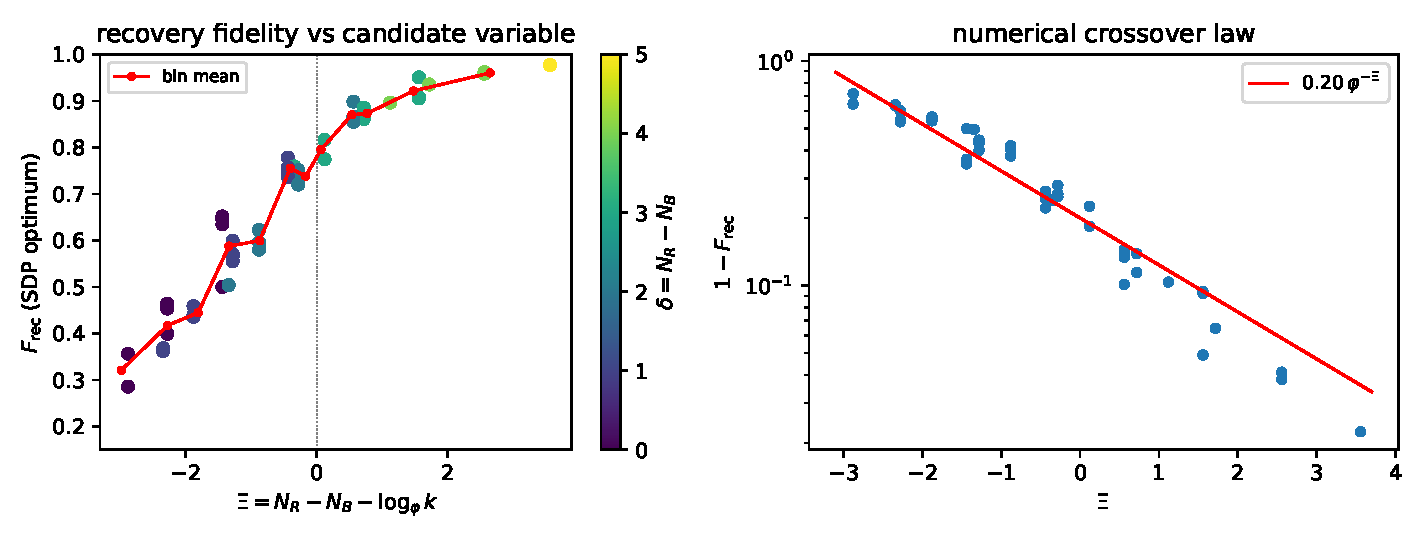
\includegraphics[width=0.98\textwidth]{fig_collapse.pdf}
\caption{左：CPTP 最优 $F_{\rm rec}$ 对候选变量 $\Xi=N_R-N_B-\log_\ph k$（颜色为 $\delta=N_R-N_B$）；红线为分箱均值。右：$1-F_{\rm rec}$ 对 $\Xi$ 的半对数图（红实线为经验律 $0.20\,\ph^{-\Xi}$）。数据含 49 组 $(N_R,N_B,k)$。}
\label{fig:collapse}
\end{figure}

\begin{figure}[t]\centering
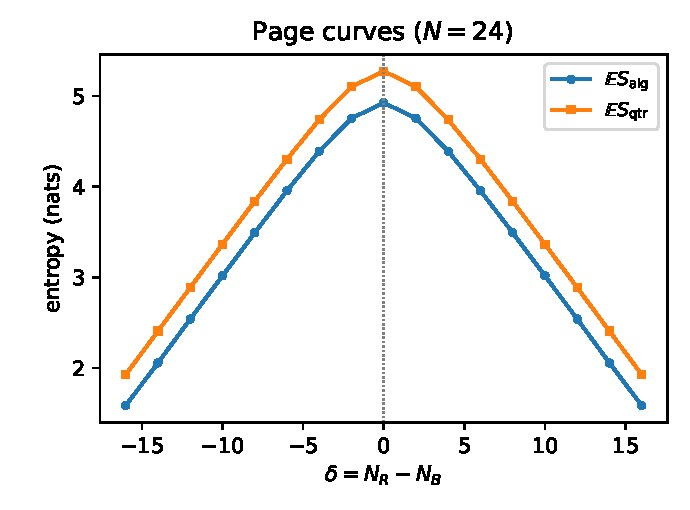
\includegraphics[width=0.55\textwidth]{fig_page.pdf}
\caption{精确期望熵的 Page 曲线（$N=24$，横轴 $\delta=N_R-N_B$）：$S_{\rm alg}$ 与 $S_{\rm qtr}$ 的转折都在 $\delta=0$，两者相差常数 $p_\tau^\star\log\ph=0.3482$。}
\label{fig:page}
\end{figure}

\subsection{候选临界变量的检验}

定义单参数族 $\Xi_\alpha:=N_R-N_B-\alpha\log_\ph k$，对 $1-F_{\rm SDP}\in(0.015,0.75)$ 的点做最小二乘
$\log(1-F)=a-b\,\Xi_\alpha$（理想斜率 $b=\log\ph=0.4812$）：

\begin{center}
\begin{tabular}{lllll}
\toprule
变量 & 斜率 $b$ & 常数 $c=\ee^{a}$ & rms$(\log)$ & 结论{}\\
\midrule
$\Xi_{0}$（无 $k$） & $0.5354$ & $0.598$ & $0.4475$ & 差 \\
$\Xi_{0.5}$ & $0.5758$ & $0.344$ & $0.2834$ & 差 \\
$\Xi_{1.0}$（候选） & $0.5493$ & $0.187$ & $\mathbf{0.1736}$ & \textbf{最好（或与下一行相当）}\\
$\Xi_{1.25}$ & $0.5207$ & $0.143$ & $\mathbf{0.1662}$ & 最好{}\\
$\Xi_{1.5}$ & $0.4876$ & $0.114$ & $0.1882$ & 尚可{}\\
$\Xi_{2.0}$ & $0.4191$ & $0.081$ & $0.2619$ & 差{}\\
\midrule
$N_R-\log_\ph k$ & $0.3793$ & $0.736$ & $0.6271$ & 很差{}\\
$N_R-2\log_\ph k$ & $0.2974$ & $0.306$ & $0.6115$ & 很差{}\\
$\log_\ph\frac{D_R}{kD_B}$（精确维数版） & $0.5558$ & $0.184$ & $0.1816$ & 相当{}\\
\bottomrule
\end{tabular}
\end{center}

\noindent 结论：\numeric{}
\begin{enumerate}[leftmargin=1.6em]
\item 数据强烈支持系数 $\alpha=1$（即候选变量 $\Xi=N_R-N_B-\log_\ph k$）；$\alpha=0$（不含 $k$）与 $\alpha=2$ 明显更差，且不含 $N_B$ 的变量最差。精确维数版 $\log_\ph(D_R/(kD_B))$ 与 $\Xi$ 表现相当（两者仅差 $O(1/\sqrt5)$ 的格点修正），与 $kD_B\ll D_R$ 的 decoupling 判据一致。
\item 在 $N\ge11$ 的 8 个点上，$1-F_{\rm SDP}=c\,\ph^{-\Xi}$ 给出高度一致的
\begin{equation}\label{eq:law}
\boxed{\ 1-\Frec\approx 0.20\,\ph^{-\Xi},\qquad c=0.200\pm0.019\ }
\end{equation}
这是一个经验 crossover law：恢复保真度由 $\ph^{-\Xi}$ 单一控制，crossover 窗口为 $\Xi=O(1)$（具体地，$1-F=0.1$ 对应 $\Xi\approx1.33$）。
\item 启发式链条 $1-F\approx0.38\|C\|_1^2$、$\|C\|_1^2\approx0.71\,kD_B\Tr C^2$、$kD_B\Tr C^2\approx\frac{2\ph^2}{5}\ph^{-\Xi}$ 给出 $c_{\rm heur}\approx0.28$，与 \eqref{eq:law} 同阶；常数差异被标为未闭合步骤（需要更精细的谱分析）。
\end{enumerate}

\begin{conjecture}\conj{} 在 $N\to\infty$、$\Xi$ 固定于有界窗口的整数子序列上，$F_{\rm rec}(V)$ 依概率收敛到仅依赖 $\Xi$ 的极限（或在该窗口内保持 $O(1)$ 宽度），且 $1-F_{\rm rec}\asymp\ph^{-\Xi}$ 上下有界。本报告的数值只覆盖 $\Xi\in[-2.9,3.6]$、$N\le17$，不足以判定极限分布。
\end{conjecture}

\subsection{回答题面的三个具体问题}

\paragraph{(1) 两种熵的 Page 转折能否单独决定 $F_{\rm rec}$ 的转折？}
\textbf{不能。} 两种熵的转折都在 $N_R=N_B$（注~\ref{rem:page}、图~\ref{fig:page}），且位置不随 $k$ 移动；而恢复转折在 $\Xi=O(1)$，即
$N_R-N_B\approx\log_\ph k+O(1)$。二者只在 $k\to1$（单维逻辑系统）时重合到同一 $O(1)$ 窗口；对 $k\ge2$，两者相差 $\log_\ph k$。
数值上：在 Page 点 $\delta=0$ 处（$k=2$）有 $F_{\rm rec}\approx0.63\text{--}0.65$（$(3,3),(4,4),(5,5),(6,6)$：$0.635,0.649,0.646,0.652$），明显未达到高保真恢复；而 $\delta\gtrsim3$ 后（如 $(5,2,k=2)$：$F=0.951$；$(6,2,k=2)$：$F=0.959$）才进入恢复区。因此熵曲线形状无法替代信道层的 decoupling 分析。

\paragraph{(2) $d_\tau$、扇区权重、融合重数分别在哪一步进入可操作信息恢复？哪些只改变 entropy convention、哪些改变信道？}
\begin{itemize}[leftmargin=1.6em]
\item $d_\tau=\ph$ 本身\textbf{不进入}题面定义的量子信道；它只通过两种途径起作用：（i）$S_{\rm qtr}$ 的 \emph{quantum trace} 约定，贡献 $S_{\rm qtr}-S_{\rm alg}=\sum_ap_a\log d_a$（期望 $p_\tau^\star\log\ph=0.3482$），这是纯 convention 差别；（ii）作为 $m_a,n_a,D$ 的增长率 $\ph^{N}$ 出现（$\ph$ 是维数增长底数）。
\item 扇区权重 $p_a$（Dirichlet$(m_1n_1,m_\tau n_\tau)$，均值 $p_a^\star$）进入：熵分解中的经典项 $H(p)$；精确矩公式中的求和权重；经验律常数 $c$。其涨落为 $O(1/\sqrt{\alpha_a})$，不影响转折位置。经典标签泄漏 $O(\ph^{-N/2})$ 是被 $C_{QB}$ 的精确公式自动包含的次主导项。
\item 融合重数 $m_a,n_a$（Kraus 秩、输出维数、$D,D_R,D_B$）\textbf{就是信道的全部数据}：它们决定 $\E\Tr C^2$ 的精确值 \eqref{eq:main}、trace norm 标度、以及阈值 $kD_B\lesssim D_R$。在临界窗口内，只有它们的 $\ph$-增长进入指数，$F_n=(\ph^n-(-1)^n\ph^{-n})/\sqrt5$ 的 $\ph^{-2N_B}$ 修正进入常数与拟合的有限尺度漂移。
\end{itemize}

\paragraph{(3) island/QES 字典（最小对应）。}
本模型\textbf{不预设引力对偶}，下面的对应只是 $S_{\rm rad}$ 账目层面的：
\[
S_{\rm rad}\leftrightarrow S(R);\qquad
\text{``island 相’’}\ (N_R>N_B)\leftrightarrow \text{取 } \min(N_R,N_B)\log\ph \text{ 的项};
\]
\[
N_B\log\ph+\text{const}\leftrightarrow \text{``面积/岛’’贡献};
\]

而常数 $C_1=H(p^\star)-p_1^\star\log\ph$、$\ph^{-|\delta|}/2$、以及约定平移 $p_\tau^\star\log\ph$ 对应“center/edge/topological”贡献。$\ph$（量子维度）以底数形式进入“面积”$\log\dim\mathcal H_B\simeq N_B\log\ph$；bulk 熵在这一层面只能对应 $B$ 侧约化熵 $S(\rho_B)$（其 Page 值 $\approx N_B\log\ph+\text{const}$）。\textbf{缺失的动力学/编码假设}：(i) 没有哈密顿量或引力约束，random code 无法给出几何的 QES 极小化；(ii) 没有局部性与面积律结构（Haar 随机 vs 几何张量网络）；(iii) 没有 gauge 约束/边界算符代数。因此不能由熵曲线形状宣称“证明了 island”或“构造了全息对偶”；本模型只演示了 Page 转折与恢复阈值是\emph{两个独立}的物理量，这与 island 图像中“熵转折 $\neq$ 重构转折”的定性预期相容。

\section{状态清单与开放问题}
\label{sec:status}

\begin{center}
\small\setlength{\tabcolsep}{4pt}\begin{tabular}{p{0.70\textwidth}l}
\toprule
事实 & 状态{}\\
\midrule
Fibonacci 维数恒等式、$m_a,n_a,D,D_R,D_B$ & \proved\\
$\mathcal N_R,\mathcal N_B$ 为精确互补对（扇区退相干自动） & \proved\\
保切分基变换不变性 & \proved\\
$(p_1,p_\tau)\sim\mathrm{Dir}$，条件独立性 & \proved\\
$\E\Nalg,\E\Nqtr$ 的精确有限维公式 & \proved\\
$\E\Tr(\rho_R^{\rm alg})^2$ 精确公式（二阶 replica moment） & \proved\\
\eqref{eq:Sdecomp}（$S_{\rm qtr}=S_{\rm alg}+\langle\log d_a\rangle$） & \proved\\
渐近 \eqref{eq:asymS}（主项与常数项；$O(\ph^{-2N_B})$ 由数值确认） & \proved/\loword\\
$\E\Tr C_{QB}^2$ 精确公式 \eqref{eq:main} & \proved\\
渐近 \eqref{eq:asymTrC2}、\eqref{eq:asymXi}（系数由 Binet 展开） & \proved\\
Petz 下界 \eqref{eq:petz}；SDP 对偶上界 \eqref{eq:dual} & \proved\\
Markov 典型界（推论~\ref{cor:markov}） & \proved\\
$1-F\approx0.38\|C\|_1^2$、$\|C\|_1^2\approx0.71kD_B\Tr C^2$ & \numeric\\
经验律 $1-F\approx0.20\ph^{-\Xi}$（$N\ge11$） & \numeric\\
$\Xi$ 为正确临界变量（$\alpha=1$ 最优，$\alpha=0,2$ 明显更差） & \numeric\\
经典标签泄漏 $O(\ph^{-N/2})$ & \numeric\\
固定 $\Xi$ 窗口的极限分布/极限函数；严格证明 $1-F\asymp\ph^{-\Xi}$ 的上下界 & \conj\\
\bottomrule
\end{tabular}
\end{center}

\paragraph{开放问题.}
(a) 严格证明存在常数 $0<c_1<c_2$ 使 $c_1\ph^{-\Xi}\le1-F_{\rm rec}\le c_2\ph^{-\Xi}$（在 $\Xi=O(1)$ 窗口内，概率 $\to1$）；(b) 把 \eqref{eq:law} 的 $c$ 常数从第一原理定出；(c) 方差/大偏差控制（本报告只给期望与样本标准差）；(d) 渐近展开的 $O(\ph^{-2N_B})$ 系数对 $\delta$ 的显式依赖。

\begin{thebibliography}{99}
\bibitem{Page93} D.~N.~Page, \textit{Average entropy of a subsystem}, Phys.\ Rev.\ Lett.\ \textbf{71}, 1291 (1993).
\bibitem{FK94} S.~K.~Foong, S.~Kanno, \textit{Proof of Page's conjecture on the average entropy of a subsystem}, Phys.\ Rev.\ Lett.\ \textbf{72}, 1148 (1994).
\bibitem{Lubkin78} E.~Lubkin, \textit{Entropy of an $n$-system from its correlation with a $k$-reservoir}, J.\ Math.\ Phys.\ \textbf{19}, 1028 (1978).
\bibitem{Petz86} D.~Petz, \textit{Sufficient subalgebras and the relative entropy of states of a von Neumann algebra}, Commun.\ Math.\ Phys.\ \textbf{105}, 123 (1986).
\bibitem{SN96} B.~Schumacher, M.~A.~Nielsen, \textit{Quantum data processing and error correction}, Phys.\ Rev.\ A \textbf{54}, 2629 (1996).
\bibitem{BK02} H.~Barnum, E.~Knill, \textit{Reversing quantum dynamics with near-optimal quantum and classical fidelity}, J.\ Math.\ Phys.\ \textbf{43}, 2097 (2002).
\bibitem{KL97} E.~Knill, R.~Laflamme, \textit{Theory of quantum error-correcting codes}, Phys.\ Rev.\ A \textbf{55}, 900 (1997).
\bibitem{DBWR14} F.~Dupuis, M.~Berta, J.~Wullschleger, R.~Renner, \textit{One-shot decoupling}, Commun.\ Math.\ Phys.\ \textbf{328}, 251 (2014).
\bibitem{Weingarten} B.~Collins, P.~\'Sniady, \textit{Integration with respect to the Haar measure on unitary, orthogonal and symplectic group}, Commun.\ Math.\ Phys.\ \textbf{264}, 773 (2006).
\bibitem{Kitaev03} A.~Kitaev, \textit{Fault-tolerant quantum computation by anyons}, Ann.\ Phys.\ \textbf{303}, 2 (2003).
\bibitem{TW08} S.~Trebst, M.~Troyer, Z.~Wang, A.~W.~W.~Ludwig, \textit{A short introduction to Fibonacci anyon models}, Prog.\ Theor.\ Phys.\ Suppl.\ \textbf{176}, 384 (2008).
\bibitem{HP07} P.~Hayden, J.~Preskill, \textit{Black holes as mirrors: quantum information in random subsystems}, JHEP \textbf{09}, 120 (2007).
\bibitem{Pen19} G.~Penington, \textit{Entanglement wedge reconstruction and the information paradox}, JHEP \textbf{09}, 002 (2020).
\bibitem{AEM19} A.~Almheiri, N.~Engelhardt, D.~Marolf, H.~Maxfield, \textit{The entropy of bulk quantum fields and the entanglement wedge of an evaporating black hole}, JHEP \textbf{12}, 063 (2019).
\bibitem{AHMS20} A.~Almheiri, T.~Hartman, J.~Maldacena, E.~Shaghoulian, A.~Tajdini, \textit{Replica wormholes and the entropy of Hawking radiation}, JHEP \textbf{05}, 013 (2020).
\bibitem{Wilde} M.~M.~Wilde, \textit{Quantum Information Theory}, 2nd ed., Cambridge University Press (2017)（Haar 积分、transpose/Petz 信道、decoupling 与 Page 曲线的教材处理）.
\end{thebibliography}

\appendix

\section{矩计算的完整中间步骤}
\label{app:proof}

记 $w_{(a\mu\nu)j}:=X_a^{(j)}{}_{\mu\nu}$，$D:=D_N$。由引理~\ref{lem:moment}，四指标矩只依赖行指标配对与列指标配对。

\paragraph{$T_1$ 的收缩。}
$T_1=\E\sum_a\sum_{j,l}\sum_{\mu_1\mu_2}\sum_{\nu_1\nu_2}\bar w_{(\mu_1\nu_1)j}w_{(\mu_1\nu_2)l}w_{(\mu_2\nu_1)j}\bar w_{(\mu_2\nu_2)l}$。按 \eqref{eq:moment}：
\begin{align*}
\mathbb E[\ldots]=&\ \frac{1}{D^2-1}\Big[\delta_{r_2r_1}\delta_{r_3r_4}\delta_{jl}+\delta_{r_2r_4}\delta_{r_3r_1}\Big]
-\frac{1}{D(D^2-1)}\Big[\delta_{r_2r_1}\delta_{r_3r_4}+\delta_{r_2r_4}\delta_{r_3r_1}\delta_{jl}\Big],
\end{align*}
其中 $r_1=(\mu_1\nu_1),r_2=(\mu_1\nu_2),r_3=(\mu_2\nu_1),r_4=(\mu_2\nu_2)$，故
$\delta_{r_2r_1}=\delta_{r_3r_4}=\delta_{\nu_1\nu_2}$，$\delta_{r_2r_4}=\delta_{r_3r_1}=\delta_{\mu_1\mu_2}$。求和得
\[
\E[\ldots]=\frac{\delta_{\nu_1\nu_2}\delta_{jl}+\delta_{\mu_1\mu_2}}{D^2-1}
-\frac{\delta_{\nu_1\nu_2}+\delta_{\mu_1\mu_2}\delta_{jl}}{D(D^2-1)} .
\]
对 $(\mu_1,\mu_2,\nu_1,\nu_2,j,l)$ 求和：\[
\textstyle\sum\delta_{\nu_1\nu_2}\delta_{jl}=m_a^2n_ak,\quad
\sum\delta_{\mu_1\mu_2}=m_an_a^2k^2,\quad
\sum\delta_{\nu_1\nu_2}=m_a^2n_ak^2,\quad
\sum\delta_{\mu_1\mu_2}\delta_{jl}=m_an_a^2k,
\]
，即 \eqref{eq:T1}。

\paragraph{$T_2$ 的收缩。}
$\Tr\rho_B^2=\frac1{k^2}\sum_{j,l}\Tr(O_{jj}O_{ll})$，且
$\Tr(O_{jj}O_{ll})=\sum_a\Tr\big(X_a^{(j)\dagger}X_a^{(j)}X_a^{(l)\dagger}X_a^{(l)}\big)$（引理~\ref{lem:trace} 的同类展开；亦可用 $\overline{X^\dagger X}$ 的厄米性）。对
\[
\bar w_{(\mu\nu)j}w_{(\mu\nu')j}\bar w_{(\mu'\nu')l}w_{(\mu'\nu)l}
\]
 用同一矩公式，得
$\frac{\delta_{\nu\nu'}^2+\delta_{\mu\mu'}^2\delta_{jl}}{D^2-1}-\frac{\delta_{\nu\nu'}^2\delta_{jl}+\delta_{\mu\mu'}^2}{D(D^2-1)}$，求和给出 \eqref{eq:T2}。

\paragraph{组合。}
$kT_1-T_2=\frac{k(k^2-1)B}{D^2-1}-\frac{k(k^2-1)A}{D(D^2-1)}=k(k^2-1)\frac{DB-A}{D(D^2-1)}$，
而 $\E\Tr C^2=\Tr\rho_{QB}^2-\frac1k\Tr\rho_B^2=\frac{T_1}{k^2}-\frac{T_2}{k^3}=\frac{kT_1-T_2}{k^3}$，即 \eqref{eq:main}。

\section{数值方法与全部扫描数据}
\label{app:data}
\label{app:code}

\paragraph{数值方法} $V$ 由复 Gaussian QR 取样（Haar/Stiefel）；$\rho_{QR}$ 按分块组装。CPTP 优化 $\max\langle\Phi|(\id\otimes\mathcal D)(\rho)|\Phi\rangle$ 写成 SDP：Choi 矩阵 $J\succeq0$，$\Tr_LJ=I_R$；用 CVXPY/SCS 求解（$\varepsilon=10^{-9}$），并用 \eqref{eq:dual} 交叉校验。每格 $10$ 个样本；Petz 值用命题~\ref{prop:petz} 的闭式与显式解码两种方式互相一致。
脚本与数据在 \texttt{work/}：\texttt{scan\_recovery.py}、\texttt{sdp\_recovery.py}、\texttt{partA\_B\_montecarlo.py}、\texttt{final\_tables.py} 及 \texttt{results\_recovery.csv}。

\begin{table}[h]\centering
\caption{全部扫描结果（每格 10 个样本的均值）。$\Xi=N_R-N_B-\log_\ph k$。$F_{\rm SDP}$ 为 CPTP 最优保真度；$F_P$ 为 Petz 下界；最后两列为互补量（$Q$ 与 $R$）。}
\label{tab:scan}
\small
\begin{tabular}{cccccccccc}
\toprule
$N_R$ & $N_B$ & $k$ & $D$ & $\Xi$ & $\Tr C_{QB}^2$ & $\|C_{QB}\|_1$ & $F_{\rm SDP}$ & $F_P$ & $\|C_{QR}\|_1$\\
\midrule
3 & 3 & 4 & 5 & -2.88 & 0.28491 & 1.4814 & 0.2857 & 0.2589 & 1.4814 \\
5 & 5 & 4 & 34 & -2.88 & 0.11241 & 1.4272 & 0.3564 & 0.2890 & 1.4505 \\
4 & 3 & 5 & 8 & -2.34 & 0.16367 & 1.3203 & 0.3683 & 0.3350 & 1.7278 \\
5 & 4 & 5 & 21 & -2.34 & 0.11654 & 1.3272 & 0.3622 & 0.3245 & 1.7017 \\
3 & 3 & 3 & 5 & -2.28 & 0.26231 & 1.2934 & 0.3994 & 0.3538 & 1.2946 \\
4 & 4 & 3 & 13 & -2.28 & 0.17314 & 1.2570 & 0.4640 & 0.3789 & 1.2474 \\
5 & 5 & 3 & 34 & -2.28 & 0.11197 & 1.2538 & 0.4558 & 0.3811 & 1.2542 \\
6 & 6 & 3 & 89 & -2.28 & 0.07045 & 1.2542 & 0.4536 & 0.3821 & 1.2556 \\
4 & 3 & 4 & 8 & -1.88 & 0.15706 & 1.1538 & 0.4585 & 0.4176 & 1.6461 \\
5 & 4 & 4 & 21 & -1.88 & 0.11526 & 1.2001 & 0.4395 & 0.3964 & 1.6092 \\
6 & 5 & 4 & 55 & -1.88 & 0.07680 & 1.2078 & 0.4360 & 0.3949 & 1.6042 \\
2 & 2 & 2 & 2 & -1.44 & 0.25000 & 1.0000 & 0.5000 & 0.5000 & 1.0000 \\
3 & 3 & 2 & 5 & -1.44 & 0.25161 & 0.9786 & 0.6349 & 0.5548 & 0.9242 \\
4 & 4 & 2 & 13 & -1.44 & 0.12920 & 0.9221 & 0.6490 & 0.5834 & 0.9775 \\
5 & 5 & 2 & 34 & -1.44 & 0.09637 & 0.9526 & 0.6460 & 0.5797 & 0.9659 \\
6 & 6 & 2 & 89 & -1.44 & 0.05694 & 0.9562 & 0.6517 & 0.5820 & 0.9763 \\
5 & 3 & 5 & 13 & -1.34 & 0.10430 & 1.0411 & 0.5041 & 0.4886 & 1.8025 \\
3 & 2 & 3 & 3 & -1.28 & 0.14815 & 0.8889 & 0.5556 & 0.5556 & 1.5556 \\
4 & 3 & 3 & 8 & -1.28 & 0.15201 & 0.9539 & 0.5993 & 0.5430 & 1.4967 \\
5 & 4 & 3 & 21 & -1.28 & 0.10842 & 1.0234 & 0.5666 & 0.5242 & 1.4618 \\
6 & 5 & 3 & 55 & -1.28 & 0.07090 & 1.0184 & 0.5709 & 0.5249 & 1.4561 \\
4 & 2 & 4 & 5 & -0.88 & 0.09316 & 0.8118 & 0.6227 & 0.6227 & 1.7794 \\
5 & 3 & 4 & 13 & -0.88 & 0.10190 & 0.9138 & 0.5958 & 0.5878 & 1.7355 \\
6 & 4 & 4 & 34 & -0.88 & 0.07185 & 0.9770 & 0.5805 & 0.5666 & 1.7131 \\
3 & 2 & 2 & 3 & -0.44 & 0.13696 & 0.7223 & 0.7505 & 0.7505 & 1.2223 \\
4 & 3 & 2 & 8 & -0.44 & 0.11811 & 0.7016 & 0.7783 & 0.7611 & 1.2074 \\
5 & 4 & 2 & 21 & -0.44 & 0.09313 & 0.7909 & 0.7368 & 0.7129 & 1.1448 \\
6 & 5 & 2 & 55 & -0.44 & 0.05629 & 0.7642 & 0.7568 & 0.7323 & 1.1653 \\
7 & 6 & 2 & 144 & -0.44 & 0.03812 & 0.7901 & 0.7505 & 0.7221 & 1.1471 \\
5 & 2 & 5 & 8 & -0.34 & 0.05166 & 0.6393 & 0.7593 & 0.7593 & 1.8752 \\
4 & 2 & 3 & 5 & -0.28 & 0.09997 & 0.6897 & 0.7437 & 0.7437 & 1.6459 \\
5 & 3 & 3 & 13 & -0.28 & 0.09814 & 0.7632 & 0.7511 & 0.7409 & 1.6047 \\
6 & 4 & 3 & 34 & -0.28 & 0.06668 & 0.8091 & 0.7202 & 0.7113 & 1.5893 \\
5 & 2 & 4 & 8 & 0.12 & 0.05470 & 0.5718 & 0.8164 & 0.8164 & 1.8172 \\
6 & 3 & 4 & 21 & 0.12 & 0.06498 & 0.7323 & 0.7748 & 0.7728 & 1.7876 \\
4 & 2 & 2 & 5 & 0.56 & 0.07829 & 0.5425 & 0.8987 & 0.8987 & 1.3576 \\
5 & 3 & 2 & 13 & 0.56 & 0.08759 & 0.5934 & 0.8662 & 0.8622 & 1.3055 \\
6 & 4 & 2 & 34 & 0.56 & 0.05245 & 0.5957 & 0.8609 & 0.8567 & 1.3027 \\
7 & 5 & 2 & 89 & 0.56 & 0.03643 & 0.6166 & 0.8555 & 0.8507 & 1.2908 \\
5 & 2 & 3 & 8 & 0.72 & 0.05485 & 0.4871 & 0.8856 & 0.8856 & 1.7034 \\
6 & 3 & 3 & 21 & 0.72 & 0.05929 & 0.5866 & 0.8611 & 0.8595 & 1.6765 \\
6 & 2 & 4 & 13 & 1.12 & 0.03939 & 0.5047 & 0.8963 & 0.8963 & 1.8357 \\
5 & 2 & 2 & 8 & 1.56 & 0.04096 & 0.3732 & 0.9509 & 0.9509 & 1.4286 \\
6 & 3 & 2 & 21 & 1.56 & 0.05984 & 0.5112 & 0.9078 & 0.9066 & 1.3637 \\
7 & 4 & 2 & 55 & 1.56 & 0.03772 & 0.5067 & 0.9058 & 0.9045 & 1.3613 \\
6 & 2 & 3 & 13 & 1.72 & 0.03611 & 0.4042 & 0.9354 & 0.9355 & 1.7322 \\
6 & 2 & 2 & 13 & 2.56 & 0.03350 & 0.3479 & 0.9588 & 0.9587 & 1.4402 \\
7 & 3 & 2 & 34 & 2.56 & 0.02623 & 0.3372 & 0.9617 & 0.9615 & 1.4432 \\
7 & 2 & 2 & 21 & 3.56 & 0.01907 & 0.2452 & 0.9776 & 0.9776 & 1.4671 \\
\bottomrule
\end{tabular}
\end{table}

\end{document}
